\documentclass[15pt,uplatex,dvipdfmx]{jsarticle}
\usepackage{indentfirst}
\usepackage{tabularx}
\usepackage[hmargin=2cm,vmargin=2cm]{geometry}
\usepackage{amsmath}
\usepackage[dvips]{graphicx}
\usepackage{listings}
\usepackage{float}

%%% tabularx環境用マクロ
%%セル内で中央揃えをする。
\newcolumntype{C}{>{\centering\arraybackslash}X}
%%セル内で右揃え。
\newcolumntype{R}{>{\raggedright\arraybackslash}X}
%%セル内で左揃え。
\newcolumntype{L}{>{\raggedleft\arraybackslash}X}

\begin{document}

\setcounter{section}{6}

\section{機器配置 $\cdot$ 放熱面の決定}

\subsection{フェアリング重量の推算}
フェアリングの直径をDとする.マージンとして150mmを確保することにすると,衛星の対角線の
長さを考慮して,
\begin{equation}
  D > \sqrt{2}3.2m + 0.15m = 4.675m
\end{equation}
となり、ロケットのサイジングの配布資料よりフェアリング重量$W_F$は
\begin{equation}
  W_F = \frac{2}{4^{2.2}}D^{2.2} = 2.818t
\end{equation}
となる.

\subsection{必要$\Delta V$の計算}
必要$\Delta V$は
\begin{equation}
  \Delta V = \Delta V_{PO} + \Delta V_{PK}
\end{equation}
\begin{equation}
  \Delta V_{PO}= \text{地上からパーキング軌道までの$\Delta V$}
   =V_{CE} + \Delta V_H + \Delta V_g + \Delta V_A - \Delta V_E
\end{equation}
\subsubsection{$V_{CE}$}
これは高度0kmにおける円軌道速度であり,地球の半径6371kmを用いると
\begin{equation}
  V_{CE} = \sqrt{\frac{\mu}{R}}
  = \sqrt{\frac{3.986\times 10^{14}}{6371\times 10^3}}
   = 7909.8m/s
\end{equation}
となる.
\subsubsection{$\Delta V_H$}
これは高度0kmの円軌道から半径6600kmの円軌道に至るホーマン移行の$\Delta V$である.
パーキング円軌道での速度$V_{PO}$は
\begin{equation}
V_{PO} =  \sqrt{\frac{\mu}{R_{PO}}}
 = \sqrt{\frac{3.986\times 10^{14}}{6600\times 10^3}}
  = 7771.4m/s
\end{equation}
ホーマン遷移軌道のアポジ点とペリジ点における速度は
\begin{equation}
V_{H@APG} =  \sqrt{\frac{2\mu R_E}{R_{PO}(R_E+R_{PO})}}=7702.4m/s
\end{equation}
\begin{equation}
V_{H@PRG} =  \sqrt{\frac{2\mu R_{PO}}{R_E(R_E+R_{PO})}}=7979.3m/s
\end{equation}
であるから,
\begin{equation}
  \Delta V_H = (V_{H@PRG} - V_{CE}) + (V_{PO} -V_{H@APG}) =138.5m/s
\end{equation}
\subsubsection{$\Delta V_g$と$\Delta V_A$}
これはグラビティ・ロスと空気抵抗による損失である.
\begin{equation}
  \Delta V_g + \Delta V_A = 1680m/s
\end{equation}
\subsubsection{$\Delta V_E$}
これは地球自転による速度であり,緯度$30^\circ$として,
\begin{equation}
  \Delta V_E = 400m/s
\end{equation}
\subsubsection{$\Delta V_{PK}$}
これはGTO投入時のペリジキックの時の値であり,
\begin{equation}
  V_{GTO@PRG} =  \sqrt{\frac{2\mu R_{GEO}}{R_GEO(R_{PO}+R_{GEO})}}=10219.4m/s
\end{equation}
となるので
\begin{equation}
  \Delta V_{PK} = V_{GTO@PRG} - V_{PO} = 2448.1m/s
\end{equation}

\subsection{$\Delta V$の合計}
\begin{equation}
  \Delta V_{PO} =V_{CE} + \Delta V_H + \Delta V_g + \Delta V_A - \Delta V_E = 11776m/s
\end{equation}

\subsection{1・2段ロケットの推進薬の決定}
自分たちの班は,液酸液水ロケットを設計した。配布プリントの液体水素,液体酸素
の$I_sp$の値を用いる.

1段目では
\begin{equation}
  I_{sp} = 430s
\end{equation}

2段目では
\begin{equation}
 I_{sp} = 455s
 \end{equation}
を用いることにする.

\subsection{燃料のトータル重量の最適化}
配布プリントより
\begin{equation}
  \Delta V = g(I_{sp1}log(\frac{1}{1-\xi_1}) + I_{sp2}log(\frac{1}{1-\xi_2}))
\end{equation}
\begin{equation}
 \xi_2 = \frac{0.975W_{P2}}{W_{PL} + W_{A2} + \eta_2 W_{P2} + W_{P2}}
\end{equation}
\begin{equation}
\xi_1 = \frac{0.995W_{P1}}{W_{PL} +W_2 + W_F + W_{A1} + \eta_1 W_{P1} + W_{P1}}
\end{equation}
$\eta$について配布資料の片対数グラフを直線近似して考える.
$W_P=100$のとき,$\eta = 0.105$であり,$W_P=1000$のとき,$\eta = 0.085$であることより,
通る2点が決まったので直線の方程式は
\begin{equation}
  \eta_i = -0.02 \log_{10} W_{Pi} + 0.145
\end{equation}
となる.

Chapter5の結果と設定条件より
\begin{equation}
  W_{PL} = W_{GTO} = 3203.1kg
\end{equation}
\begin{equation}
  W_{A1} = 200kg
\end{equation}
\begin{equation}
  W_{A2} = 400kg
\end{equation}
である.
また
\begin{equation}
  W_{1} = W_{A1} + \eta_1 W_{P1} + W_{P1} = 0.2 + (1.145 - 0.02 log_{10} W_{P1})W_{P1} [t]
\end{equation}
\begin{equation}
  W_{2} = W_{A2} + \eta_1 W_{P2} + W_{P2} = 0.4 + (1.145 - 0.02 log_{10} W_{P2})W_{P2} [t]
\end{equation}
フェアリング重量$W_F$は以前の議論により
\begin{equation}
  W_F = 2.818t
\end{equation}
\begin{equation}
 \xi_2 = \frac{0.975W_{P2}}{3.611 + (1.145 - 0.02 log_{10} W_{P2})W_{P2}}
\end{equation}

\begin{equation}
\xi_1 = \frac{0.995W_{P1}}{6.229 +(1.145 - 0.02 log_{10} W_{P2})W_{P2} + (1.145 - 0.02 log_{10} W_{P1})W_{P1}}
\end{equation}

式(8.17)に$\xi_1$と$\xi_2$を代入すると,$W_{P1}$と$W_{P2}$の関係式になる.
これより2段目の燃料重量から1段の燃料重量を計算する.
その結果とソースコードは以下の通り.
横軸は$W_{P2}$で縦軸は$W_{P1}$である.

\begin{figure}[H]
  \caption{機器配置図(水平方向)}
\begin{center}
  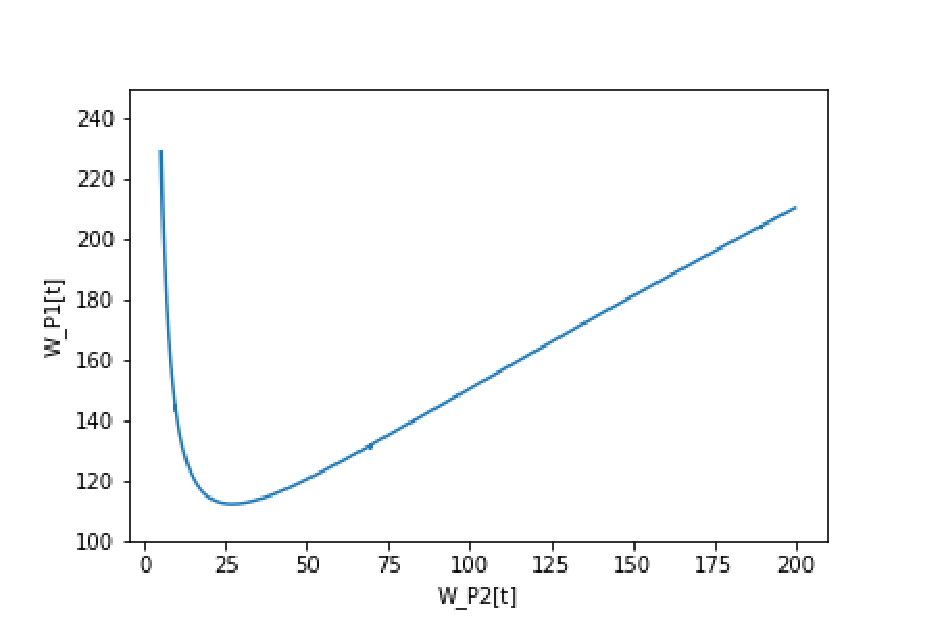
\includegraphics{saitekika0.eps}
\end{center}
\end{figure}
\newpage

\begin{lstlisting}[basicstyle=\ttfamily\footnotesize, frame=single]

  import matplotlib.pyplot as plt
  import math
  import numpy as np

  W_P2 = np.linspace(5, 200, 7000)
  W_P1 = np.array([])


  def cal_xi2(w_p2):
      return 0.975 * w_p2 / (3.611 + (1.145 - 0.02 * math.log10(w_p2)) * w_p2)


  def cal_xi1(w_p1, w_p2):
      return 0.995 * w_p1 / (6.299 + (1.145 - 0.02 * math.log10(w_p2)) *
      w_p2 + (1.145 - 0.02 * math.log10(w_p1)) * w_p1)


  def delta(w_p1, w_p2):
      return 11776 - 9.8 * (430 * math.log(1 / (1 - cal_xi1(w_p1, w_p2))) +
                            455 * math.log(1 / (1 - cal_xi2(w_p2))))


  a_list = [10, 1000]

  for j in W_P2:
      while(delta(a_list[0], j) >= 0 and delta(a_list[1], j) <= 0):
          if(abs(delta(a_list[1], j)) > 0.001):
              if(delta((a_list[0] + a_list[1]) / 2, j) > 0):
                  a_list[0] = (a_list[0] + a_list[1]) / 2
              if(delta((a_list[0] + a_list[1]) / 2, j) < 0):
                  a_list[1] = (a_list[0] + a_list[1]) / 2

          else:
              print(delta((a_list[0] + a_list[1]) / 2, j))
              print(a_list)
              W_P1 = np.append(W_P1, [(a_list[0] + a_list[1]) / 2])
              a_list = [10, 1000]
              break

  plt.plot(W_P2, W_P1)
  plt.xlabel("W_P2[t]")
  plt.ylabel("W_P1[t]")
  plt.show()

\end{lstlisting}

また打ち上げ総重量
\begin{equation}
W_0 = W_{PL} + W_F + W_1 + W_2
   = 5.327 +(1.145 - 0.02 log_{10} W_{P2})W_{P2} + (1.145 - 0.02 log_{10}) W_{P1}
\end{equation}
であり,直前の議論で$W_{P1}$と$W_{P2}$のペアの値が計算できるので
それを用いて$W_0$の最適化を行うと結果とソースコードは以下の通り.
横軸は$W_{P2}$で縦軸は$W_{P0}$である.

\begin{figure}[H]
\begin{center}
  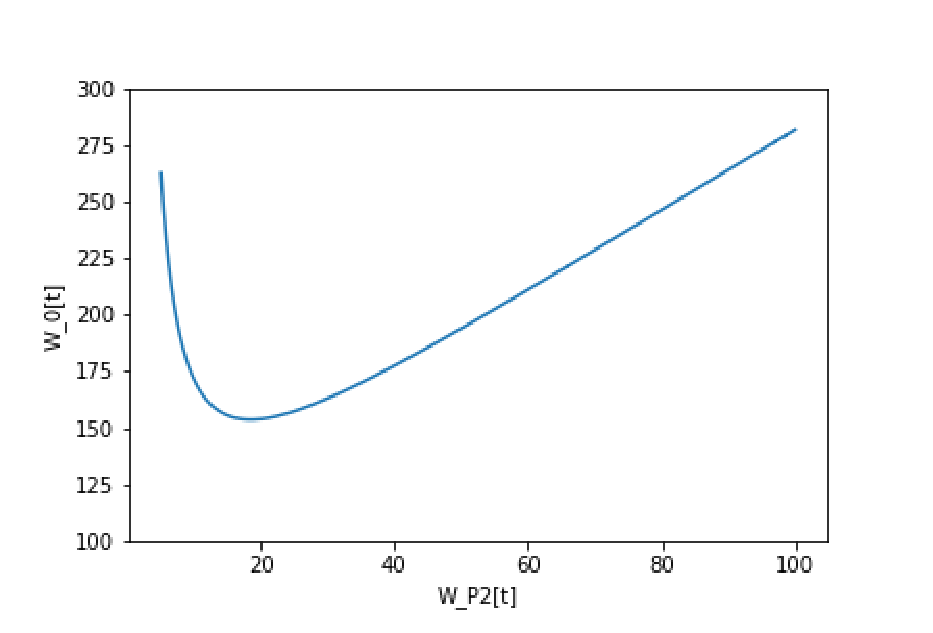
\includegraphics{saitekika.eps}
\end{center}
\end{figure} \newpage

\begin{lstlisting}[basicstyle=\ttfamily\footnotesize, frame=single]

  import matplotlib.pyplot as plt
  import math
  import numpy as np

  W_P2 = np.linspace(5, 100, 7000)
  W_P1 = np.array([])
  W_0 = np.array([])


  def cal_xi2(w_p2):
      return 0.975 * w_p2 / (3.611 + (1.145 - 0.02 * math.log10(w_p2)) * w_p2)


  def cal_xi1(w_p1, w_p2):
      return 0.995 * w_p1 / (6.299 + (1.145 - 0.02 * math.log10(w_p2)) *
       w_p2 + (1.145 - 0.02 * math.log10(w_p1)) * w_p1)


  def delta(w_p1, w_p2):
      return 11776 - 9.8 * (430 * math.log(1 / (1 - cal_xi1(w_p1, w_p2))) +
                            455 * math.log(1 / (1 - cal_xi2(w_p2))))


  a_list = [10, 1000]

  for j in W_P2:
      while(delta(a_list[0], j) >= 0 and delta(a_list[1], j) <= 0):
          if(abs(delta(a_list[1], j)) > 0.001):
              if(delta((a_list[0] + a_list[1]) / 2, j) > 0):
                  a_list[0] = (a_list[0] + a_list[1]) / 2
              if(delta((a_list[0] + a_list[1]) / 2, j) < 0):
                  a_list[1] = (a_list[0] + a_list[1]) / 2

          else:
              W_P1 = np.append(W_P1, [(a_list[0] + a_list[1]) / 2])
              W_0 = np.append(W_0, [5.327 + (1.145 - 0.02 * math.log10(j))
               * j + (1.145 - 0.02 * math.log10((a_list[0] + a_list[1]) / 2))
                * (a_list[0] + a_list[1]) / 2])

              a_list = [10, 1000]
              break

  print(np.min(W_0))
  num = np.argmin(W_0)
  print(W_P1[num])
  print(W_P2[num])
  plt.plot(W_P2, W_0)
  plt.xlabel("W_P2[t]")
  plt.ylabel("W_0[t]")
  plt.show()
\end{lstlisting}

\begin{equation}
  W_{0min} = 153.72t
\end{equation}
この時,
\begin{equation}
  W_{P1} = 115.87t
\end{equation}
\begin{equation}
  W_{P2} = 18.315t
\end{equation}
最後にこの時のペイロード比は
\begin{equation}
  \Lambda =\frac{3.203}{153.72} = 0.0208
\end{equation}
となる.
これは一般的な値に比べて小さくなってしまったが、衛星のサイズが大きいことやIspの値が
大きいことが原因として考えられる。

\end{document}
